\documentclass[12pt]{book}
\usepackage{fontspec}
\setmainfont{TeX Gyre Pagella}
\usepackage[paperwidth=8in,paperheight=8in,margin=0.6in]{geometry}
\usepackage{xcolor}
\usepackage{amssymb}
\usepackage{tikz}
\usetikzlibrary{arrows.meta}
\usetikzlibrary{patterns}
\pagestyle{empty}
\setlength{\parindent}{0pt}

\newcommand{\artnote}[1]{{\color{gray!70}\small\itshape [Illustration: #1]}\par\vspace{0.3in}}
\newcommand{\bigline}[1]{{\Huge #1}\par}
\newcommand{\pagenum}[1]{\vfill{\color{gray!50}\footnotesize #1}}
\newcommand{\sprollpage}{\newpage\vspace*{0.4in}}

\begin{document}

\thispagestyle{empty}
\begin{center}
\vspace*{1.1in}
{\Huge \textbf{SPROLL 05}}\\[0.4in]
{\huge \textbf{Together}}\\[0.5in]
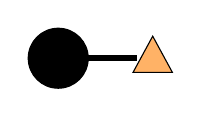
\begin{tikzpicture}
\filldraw[fill=black] (-0.6,0) circle (0.15in);
\draw[fill=orange!60] (0.35,-0.18) -- (0.6,0.28) -- (0.85,-0.18) -- cycle;
\draw[line width=2pt] (-0.45,0) -- (0.4,0);
\end{tikzpicture}
\\[0.4in]
{\large \textit{coupled, but not the same}}\\[0.3in]
{\small The Sproll Curriculum $\cdot$ Cycle I: Pops}
\end{center}

\sprollpage
\begin{center}
\vspace*{1.5in}
{\Large The Sproll Curriculum}\\[0.2in]
{\normalsize Cycle I --- Pops: Things, Differences, and Counting}\\[0.6in]
{\small Sproll 05 of 40 \quad $\cdot$ \quad follows Sproll 04: Not This Way}
\end{center}
\pagenum{2}

\sprollpage
\begin{center}
\vspace*{0.7in}
\artnote{two dots sitting near each other but with a visible gap between them, clearly separate}

\begin{tikzpicture}
\filldraw[fill=black] (-0.8,0) circle (0.15in);
\filldraw[fill=black] (0.8,0) circle (0.15in);
\end{tikzpicture}
\vspace{0.35in}
\bigline{Two Pops, sitting near each other.}
\end{center}
\pagenum{3}

\sprollpage
\begin{center}
\vspace*{0.7in}
\artnote{the same two dots, now with a clear solid line drawn between them, connecting them}
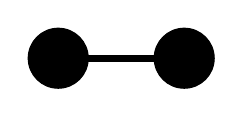
\begin{tikzpicture}
\filldraw[fill=black] (-0.8,0) circle (0.15in);
\filldraw[fill=black] (0.8,0) circle (0.15in);
\draw[line width=2.5pt] (-0.65,0) -- (0.65,0);
\end{tikzpicture}
\vspace{0.35in}
\bigline{Now they are together.}
\end{center}
\pagenum{4}

\sprollpage
\begin{center}
\vspace*{0.8in}
\artnote{the same connected pair, with a small magnifying glass hovering over one of the dots}
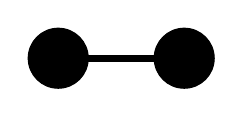
\begin{tikzpicture}
\filldraw[fill=black] (-0.8,0) circle (0.15in);
\filldraw[fill=black] (0.8,0) circle (0.15in);
\draw[line width=2.5pt] (-0.65,0) -- (0.65,0);
\end{tikzpicture}
\vspace{0.35in}
\bigline{Did they become one dot?}
\end{center}
\pagenum{5}

\sprollpage
\begin{center}
\vspace*{0.7in}
\artnote{the same connected pair, but now the two dots are pulled slightly apart to show they are still clearly two separate dots, the line stretching between them}
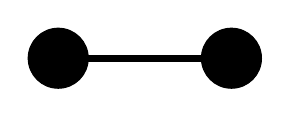
\begin{tikzpicture}
\filldraw[fill=black] (-1.1,0) circle (0.15in);
\filldraw[fill=black] (1.1,0) circle (0.15in);
\draw[line width=2.5pt] (-0.95,0) -- (0.95,0);
\end{tikzpicture}
\vspace{0.35in}
\bigline{No. Still two dots.}
\end{center}
\pagenum{6}

\sprollpage
\begin{center}
\vspace*{0.6in}
\artnote{one dot moving, dragging the connecting line and the second dot along with it, as if tied together}
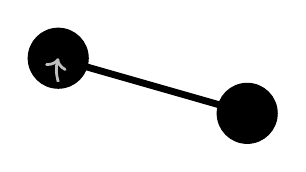
\begin{tikzpicture}
\filldraw[fill=black] (-1.3,0.4) circle (0.15in);
\filldraw[fill=black] (1.1,-0.3) circle (0.15in);
\draw[line width=2.5pt] (-1.15,0.35) -- (0.95,-0.25);
\draw[->, gray!50, line width=1pt] (-1.3,0.1) to[bend left=15] (-1.3,0.4);
\end{tikzpicture}
\vspace{0.35in}
\bigline{Move one, and the line follows.}
\end{center}
\pagenum{7}

\sprollpage
\begin{center}
\vspace*{0.7in}
\artnote{two dots with no line between them at all, sitting near each other by pure accident}
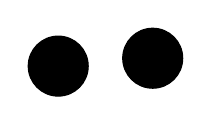
\begin{tikzpicture}
\filldraw[fill=black] (-0.6,0) circle (0.15in);
\filldraw[fill=black] (0.6,0.1) circle (0.15in);
\end{tikzpicture}
\vspace{0.35in}
\bigline{These two are just nearby.}\vspace{0.1in}
{\Large Not together. No line.}
\end{center}
\pagenum{8}

\sprollpage
\begin{center}
\vspace*{0.5in}
\artnote{a ledger entry showing two dots and a connecting line as a single new kind of entry, distinct from a plain Pop entry}
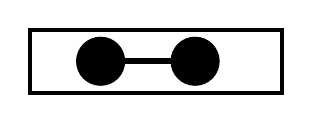
\begin{tikzpicture}
\draw[line width=1.5pt] (-1.6,-0.4) rectangle (1.6,0.4);
\filldraw[fill=black] (-0.7,0) circle (0.12in);
\filldraw[fill=black] (0.5,0) circle (0.12in);
\draw[line width=2pt] (-0.55,0) -- (0.35,0);
\end{tikzpicture}
\vspace{0.35in}
\bigline{A record can hold this too.}
\end{center}
\pagenum{9}

\sprollpage
\begin{center}
\vspace*{0.6in}
\artnote{a scale or balance beam with one dot on each side, tilting slightly, suggesting the two are linked in what happens to them}
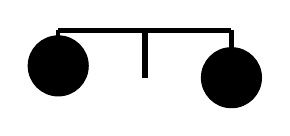
\begin{tikzpicture}
\draw[line width=2pt] (0,0) -- (0,0.6);
\draw[line width=2pt] (-1.1,0.6) -- (1.1,0.6);
\draw[line width=1.5pt] (-1.1,0.6) -- (-1.1,0.3);
\draw[line width=1.5pt] (1.1,0.6) -- (1.1,0.15);
\filldraw[fill=black] (-1.1,0.15) circle (0.15in);
\filldraw[fill=black] (1.1,0) circle (0.15in);
\end{tikzpicture}
\vspace{0.3in}
\bigline{What happens to one}\vspace{0.1in}
{\Large can matter to the other.}
\end{center}
\pagenum{10}

\sprollpage
\begin{center}
\vspace*{0.8in}
\artnote{the two connected dots, still clearly separate, each with its own small identifying mark (one striped, one plain) to emphasize they keep their own identity}
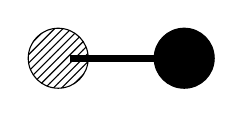
\begin{tikzpicture}
\filldraw[fill=black, pattern=north east lines] (-0.8,0) circle (0.15in);
\filldraw[fill=black] (0.8,0) circle (0.15in);
\draw[line width=2.5pt] (-0.65,0) -- (0.65,0);
\end{tikzpicture}
\vspace{0.35in}
\bigline{Each one keeps its own self.}
\end{center}
\pagenum{11}

\sprollpage
\begin{center}
\vspace*{0.6in}
\artnote{a diagram contrasting three cases side by side: two separate dots (no line), two dots merged into one (single larger dot), and two dots joined by a line -- with a checkmark under the third}
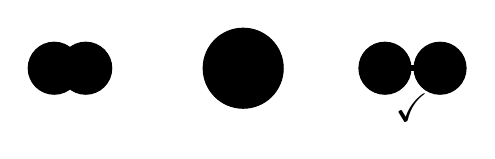
\begin{tikzpicture}
\filldraw[fill=black] (-2.4,0) circle (0.13in);
\filldraw[fill=black] (-2.0,0) circle (0.13in);
\filldraw[fill=black] (0,0) circle (0.2in);
\filldraw[fill=black] (1.8,0) circle (0.13in);
\filldraw[fill=black] (2.5,0) circle (0.13in);
\draw[line width=2pt] (1.93,0) -- (2.37,0);
\node at (2.15,-0.5) {\Large \checkmark};
\end{tikzpicture}
\vspace{0.3in}
\bigline{Not apart. Not merged.}\vspace{0.1in}
{\Large Together.}
\end{center}
\pagenum{12}

\sprollpage
\begin{center}
\vspace*{0.8in}
\artnote{a small everyday pair connected by a line -- for instance two puzzle pieces that interlock but remain two distinct pieces}
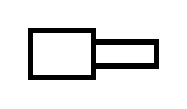
\begin{tikzpicture}
\draw[line width=2pt] (-0.8,-0.3) rectangle (0,0.3);
\draw[line width=2pt] (0,-0.15) rectangle (0.8,0.15);
\end{tikzpicture}
\vspace{0.35in}
\bigline{Two pieces. One puzzle.}\vspace{0.1in}
{\Large Still two pieces.}
\end{center}
\pagenum{13}

\sprollpage
\begin{center}
\vspace*{0.7in}
\artnote{a ledger with a Pop entry, another Pop entry, and a Bind entry connecting them, stacked as one growing history}
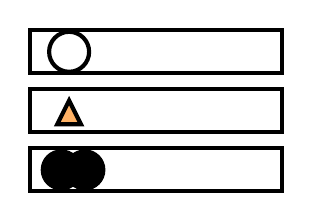
\begin{tikzpicture}
\draw[line width=1.5pt] (-1.6,0.85) rectangle (1.6,1.4);
\draw[line width=1.5pt] (-1.1,1.12) circle (0.1in);
\draw[line width=1.5pt] (-1.6,0.1) rectangle (1.6,0.65);
\draw[fill=orange!60, line width=1.5pt] (-1.25,0.2) -- (-1.1,0.5) -- (-0.95,0.2) -- cycle;
\draw[line width=1.5pt] (-1.6,-0.65) rectangle (1.6,-0.1);
\filldraw[fill=black] (-1.2,-0.38) circle (0.1in);
\filldraw[fill=black] (-0.9,-0.38) circle (0.1in);
\draw[line width=1.5pt] (-1.08,-0.38) -- (-1.02,-0.38);
\end{tikzpicture}
\vspace{0.25in}
\bigline{One record. Now three kinds of entries.}
\end{center}
\pagenum{14}

\sprollpage
\begin{center}
\vspace*{0.5in}
\artnote{a small mixed scene with several shapes -- some connected by lines, some crossed out, some plain -- viewed through a simple drawn frame or lens, as if being looked at in a particular way}
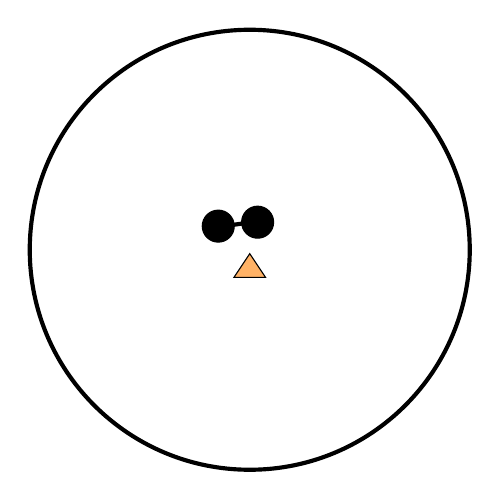
\begin{tikzpicture}
\draw[line width=1.5pt] (0,0) circle (1.1in);
\filldraw[fill=black] (-0.4,0.3) circle (0.08in);
\filldraw[fill=black] (0.1,0.35) circle (0.08in);
\draw[line width=1.5pt] (-0.32,0.3) -- (0.02,0.35);
\draw[fill=orange!60] (-0.2,-0.35) -- (0,-0.05) -- (0.2,-0.35) -- cycle;
\end{tikzpicture}
\vspace{0.3in}
\bigline{But how you look at a group}\vspace{0.1in}
{\Large can change what you see.}
\vspace{0.35in}\\
{\small \textit{--- turn the page for Sproll 06: Look Through a Rule ---}}
\end{center}
\pagenum{15}

\sprollpage
\vspace*{0.3in}
{\large \textbf{A Note for Grown-Ups}}
\vspace{0.2in}

\normalsize
This book introduces Bind: coupling two things so that what happens to one can matter to the other, without making them the same thing. Every illustration in this book takes care to keep the two bound objects visibly, physically separate, even while connected, since the temptation to picture ``together'' as ``merged into one'' is exactly the confusion this book exists to prevent.

\vspace{0.15in}
This distinction becomes important almost immediately: a later book in this series introduces a way of observing a group of things that can, under a chosen rule, treat several bound objects as a single result. That later operation, not this one, is what actually identifies things together. Bind only couples; it never merges. Keeping the two ideas separate here means a much stronger point can be made honestly later, rather than glossed over.

\vspace{0.3in}
{\small Sproll 06: Look Through a Rule continues directly from this book's final page.}
\pagenum{16}

\end{document}
